\section{HTTP-Authentifizierung}
Die Authentifizierung für HTTP soll sicherstellen, das die Anfragen eines Benutzers nur bearbeitet werden, wenn dieser dazu berechtigt ist, diese Anfragen zu stellen. Durch die Feststellung der Identität kann die Sicherheit im Netzwerk gewährleistet werden. Es gibt mehrere Arten von Methoden zur Authentifizierung. Im wesentlichen bestehen diese darin, dass der Client Benutzername und Passwort an den Server schickt, welcher diese anschließend validiert.

\paragraph{Basic Authentication}

Als am einfachsten zu Implementieren gilt das senden und überprüfen von Benutzername und Passwort im Klartext. Dies ist jedoch nur mit der Verwendung von HTTPS zu empfehlen, da die Sicherheit sonst nicht gewährleistet werden kann.

\paragraph{Digest Authentication}

Anders als bei Basic, wird das Passwort hier nicht im Klartext übertragen. Ein Hash des Passworts erhöht hier die Sicherheit und gibt somit nicht das Geheimnis preis.

\paragraph{Token-Based Authentication}

Statt eines Passworts kommt hier ein eindeutiges Token zum Einsatz, welches bei jeder Aufforderung mitgesendet wird. Der Server validiert dieses jedes mal, um die Berechtigung des Benutzers zu prüfen.

\paragraph{OAuth2 Authentication}

Der hier verwendete Token wird von einem Drittanbieter bereitgestellt, der sein eigenes Rechtesystem verwaltet. Dieser teilt dem Server bei einer Anfrage mit, ob der Benutzer berechtigt ist, auf diese Ressourcen zuzugreifen.

\section{JSON-Web-Token}
Eine mögliche Implementierung eines OAuth2 Token kann über JWT realisiert werden(bei der Erweiterung OpenIdConnect ist das immer der Fall).
Das JSON-Web-Token (JWT) setzt sich aus drei Teilen zusammen: dem Header mit Token-Typ und die Signaturmethode enthält, dem Payload, welcher Informationen über den Benutzer (z.B. E-Mail Adresse) beinhaltet und die Signatur, welche die Richtigkeit des Tokens bezeugen soll.\cite{jwt}

Ein Beispiel Token mir Inhalt kann der Abbildung \vref{jwt-decoder} entnommen werden.

\begin{figure}[ht]
	\centering
	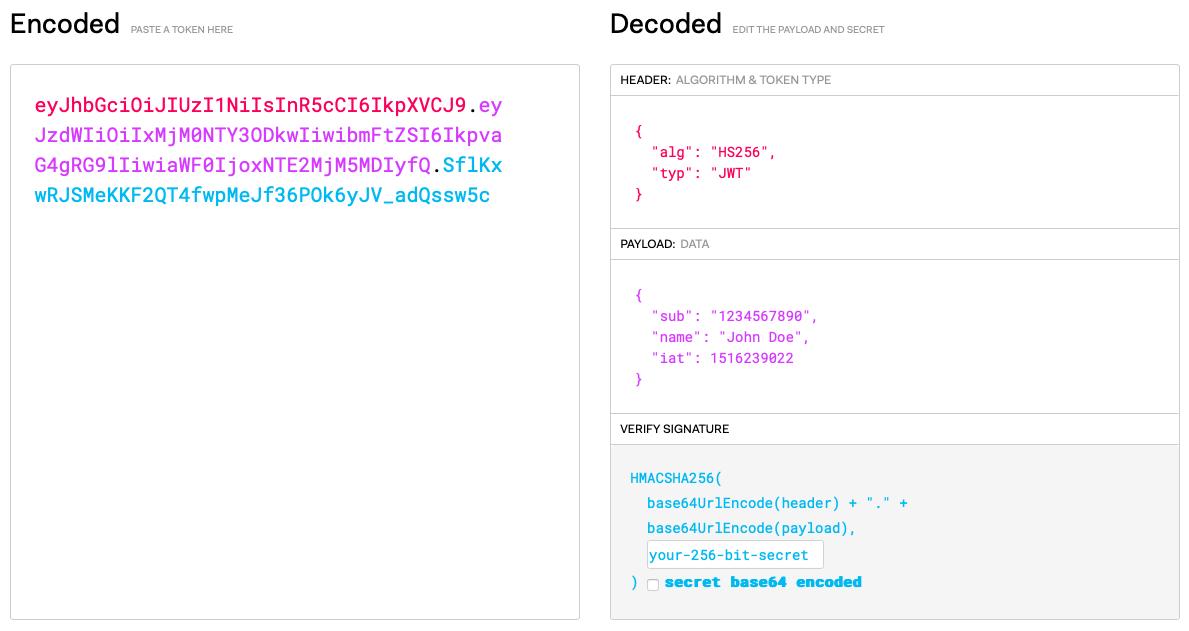
\includegraphics[width=1 \linewidth]{jwt.png}
	\caption{Vergleich von enkodiertem und dekodiertem JWT}
	\label{jwt-decoder}
\end{figure}

Dieser Standard überträgt Authentifizierungs- und Autorisierungsinformationen zwischen zwei Teilnehmern eines Netzwerks in Form einer Zeichenkette, dem Token. Diese Methode soll einen einfachen Informationsaustausch für Anmeldungen ermöglichen, ohne das eine aktive Verbindung aufrechterhalten werden muss.

Diese Eigenschaften machen JWT portabel und skalierbar. Die Übertragung ist Plattformübergreifend möglich und das Format ist kompakt. Der Server muss hier keine Sitzungsinformationen speichern, da JWT alle Informationen über die Berechtigungen enthält. Eine Manipulation ist nicht möglich, da es sonst zu Fehlern bei einer Validierung der Signatur kommt.\cite{ionos-jwt}

JWTs wirken bei Single-Sign-On (SSO) unterstützend, da der Benutzer nach einer Authentifizierung einen JWT erhält, welchen er für die Anmeldung bei Anfragen an einen Server verwenden kann.